%--------------------------------------
% Create title frame
\titleframe

%--------------------------------------
% Table of contents
\begin{frame}{Sommaire}
  \setbeamertemplate{section in toc}[sections numbered]
  \tableofcontents[hideallsubsections]
\end{frame}


%==============================================
\section{Introduction}
%==============================================

\subsection{Qu'est-ce qu'un voxel ?}

\begin{frame}[fragile=singleslide]{\insertsectionhead}
  \framesubtitle{\insertsubsectionhead}
  \vspace{0.75cm}
  \begin{figure}[ht!]
    \begin{subfigure}{0.5\textwidth}
      \frame{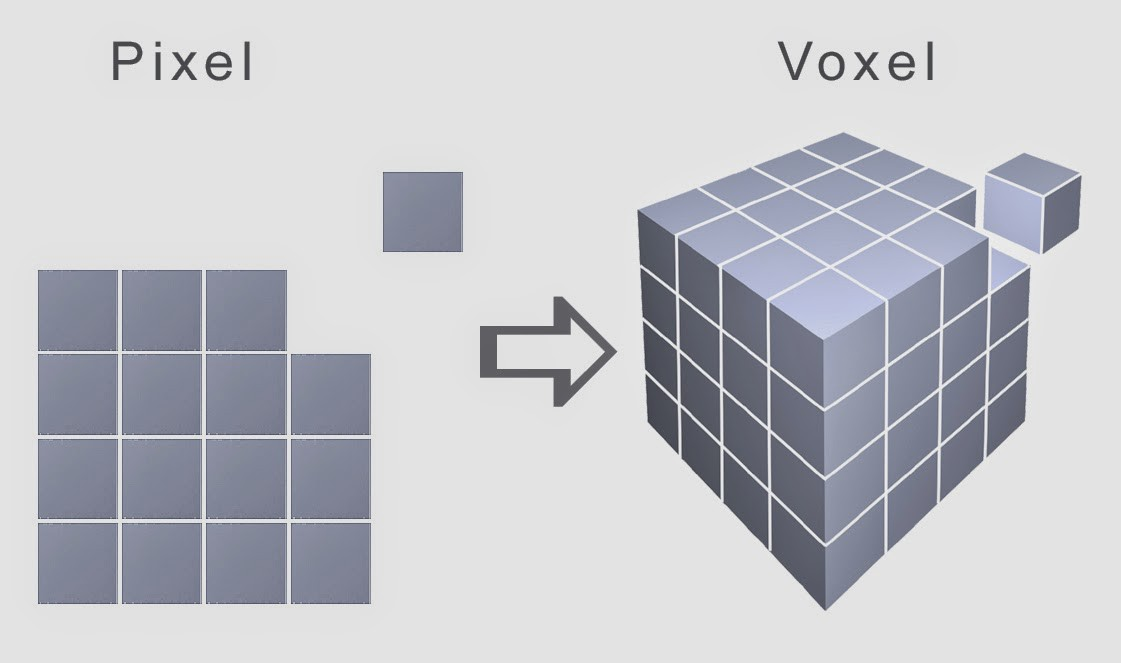
\includegraphics[width=\textwidth]{resources/voxel.jpg}}
      \caption*{Le \textbf{voxel} est à la 3D ce que le pixel est à la 2D.}
    \end{subfigure}
  \end{figure}
\end{frame}

%--------------------------------------
\subsection{Qu'est-ce que la voxelization ?}

\begin{frame}[fragile=singleslide]{\insertsectionhead}
  \framesubtitle{\insertsubsectionhead}
\end{frame}

%==============================================
\section{Etude de l'alogrithme}
%==============================================

%==============================================
\section{Prototypage \& Benchmark}
%==============================================
